Some notations used in the \autoref{fig:indis_game}:

\begin{itemize}
    \item \(pk,sk\): public-private key pair generated by the challenger.
    \item \(m\): plaintext message.
    \item \(f_b\): a specific function, where \(b\) is either 0 or 1.
    \item \(c_b\): a ciphertext encrypted using the public key \(pk\),
    where \(b\) is either 0 or 1.
    \item \(sk_{f_b}\): a functional decryption key, where \(b\) is either 0 or 1.
\end{itemize}

The indistinguishability-based security game runs as the following steps:

\begin{itemize}
    \item The adversary triggers the challenger and sends a message \(m\) such that
    \(f_0(m)=f_1(m)\).
    \item The challenger sends back the ciphertext \(c=E_{pk}(m)\) and the result of a
    random function \(f_b(m)\) wich the attacker have to guess \(b\) is 0 or 1.
    \item The adversary requests the functional key of \(f_0\)(or \(f_1\)).
    \item The challenger replies the functional key \(sk_{f_0}\) and \(sk_{f_1}\).
\end{itemize}

\begin{figure}
    \centering

    \tikzset{every picture/.style={line width=0.75pt}} %set default line width to 0.75pt        

    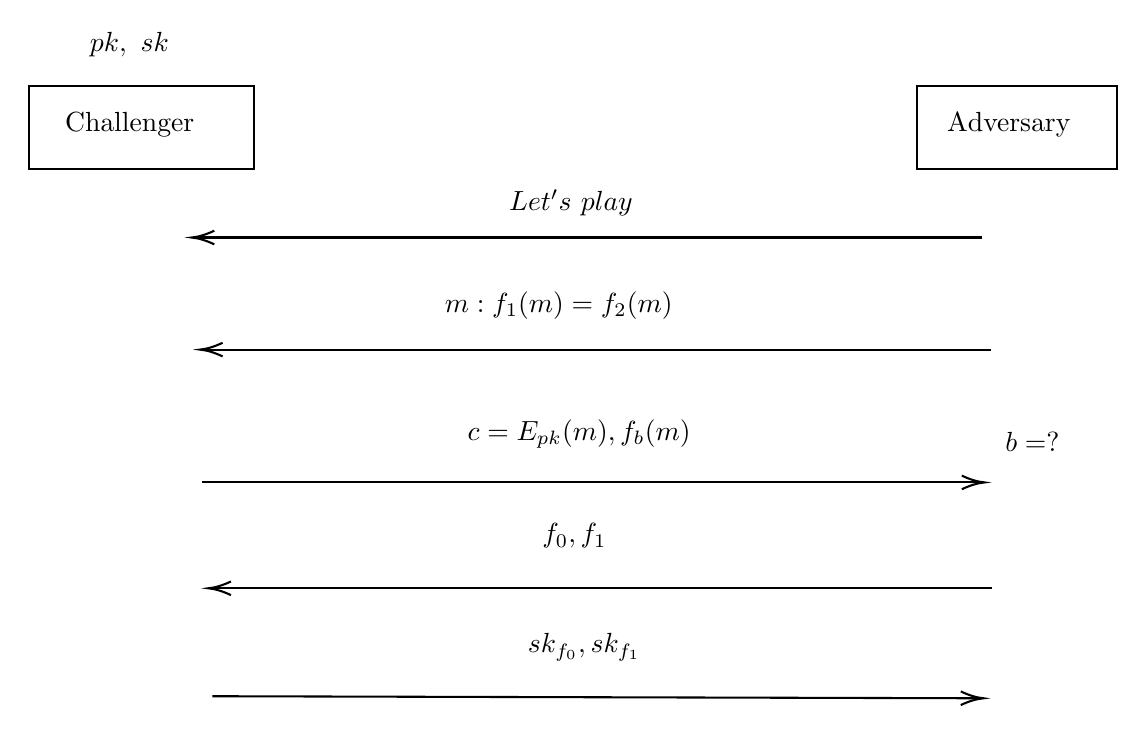
\begin{tikzpicture}[x=0.75pt,y=0.75pt,yscale=-1,xscale=1]
    %uncomment if require: \path (0,568); %set diagram left start at 0, and has height of 568

    %Shape: Rectangle [id:dp3440593711107919] 
    \draw   (61,50) -- (169.5,50) -- (169.5,90) -- (61,90) -- cycle ;

    %Shape: Rectangle [id:dp030508307813478908] 
    \draw   (489,50) -- (585.5,50) -- (585.5,90) -- (489,90) -- cycle ;

    %Straight Lines [id:da5590490769280713] 
    \draw    (520.5,123) -- (141.5,123) ;
    \draw [shift={(139.5,123)}, rotate = 360] [color={rgb, 255:red, 0; green, 0; blue, 0 }  ][line width=0.75]    (10.93,-3.29) .. controls (6.95,-1.4) and (3.31,-0.3) .. (0,0) .. controls (3.31,0.3) and (6.95,1.4) .. (10.93,3.29)   ;
    %Straight Lines [id:da19216118660880654] 
    \draw    (524.5,177) -- (145.5,177) ;
    \draw [shift={(143.5,177)}, rotate = 360] [color={rgb, 255:red, 0; green, 0; blue, 0 }  ][line width=0.75]    (10.93,-3.29) .. controls (6.95,-1.4) and (3.31,-0.3) .. (0,0) .. controls (3.31,0.3) and (6.95,1.4) .. (10.93,3.29)   ;
    %Straight Lines [id:da2103641652862146] 
    \draw    (144.5,241) -- (519.5,241) ;
    \draw [shift={(521.5,241)}, rotate = 180] [color={rgb, 255:red, 0; green, 0; blue, 0 }  ][line width=0.75]    (10.93,-3.29) .. controls (6.95,-1.4) and (3.31,-0.3) .. (0,0) .. controls (3.31,0.3) and (6.95,1.4) .. (10.93,3.29)   ;
    %Straight Lines [id:da29247082177113626] 
    \draw    (525,292) -- (149.5,292) ;
    \draw [shift={(147.5,292)}, rotate = 360] [color={rgb, 255:red, 0; green, 0; blue, 0 }  ][line width=0.75]    (10.93,-3.29) .. controls (6.95,-1.4) and (3.31,-0.3) .. (0,0) .. controls (3.31,0.3) and (6.95,1.4) .. (10.93,3.29)   ;
    %Straight Lines [id:da7797286868078096] 
    \draw    (149.5,344) -- (519,344.99) ;
    \draw [shift={(521,345)}, rotate = 180.15] [color={rgb, 255:red, 0; green, 0; blue, 0 }  ][line width=0.75]    (10.93,-3.29) .. controls (6.95,-1.4) and (3.31,-0.3) .. (0,0) .. controls (3.31,0.3) and (6.95,1.4) .. (10.93,3.29)   ;

    % Text Node
    \draw (77,61) node [anchor=north west][inner sep=0.75pt]   [align=left] {Challenger};
    % Text Node
    \draw (502,61) node [anchor=north west][inner sep=0.75pt]   [align=left] {Adversary};
    % Text Node
    \draw (291,98.4) node [anchor=north west][inner sep=0.75pt]    {$Let's\ play$};
    % Text Node
    \draw (89,22.4) node [anchor=north west][inner sep=0.75pt]    {$pk,\ sk$};
    % Text Node
    \draw (260,147.4) node [anchor=north west][inner sep=0.75pt]    {$m:f_{1}( m) =f_{2}( m)$};
    % Text Node
    \draw (271,209.4) node [anchor=north west][inner sep=0.75pt]    {$c =E_{pk}( m) ,f_{b}( m)$};
    % Text Node
    \draw (307,259.4) node [anchor=north west][inner sep=0.75pt]    {$f_{0} ,f_{1}$};
    % Text Node
    \draw (300,312.4) node [anchor=north west][inner sep=0.75pt]    {$sk_{f_{0}} ,sk_{f_{1}}$};
    % Text Node
    \draw (530,215.4) node [anchor=north west][inner sep=0.75pt]    {$b=?$};

    \end{tikzpicture}

    \caption{The indistinguishability-based security game.}\label{fig:indis_game}
\end{figure}